Предметом настоящей монографии являются детерминированные
микроструктуры~-- регулярные элементы заданной геометрии (лунки,
канавки, текстуры), описываемые явным полем добавки~$\Delta h$
в суперпозиции зазора~\eqref{eq:h_superposition} и параметризованные
в подразделе~2.2. Наряду с детерминированным рельефом любая
обработанная поверхность содержит шероховатость~-- случайную
составляющую топографии, возникающую при механической обработке,
полировке или лазерном текстурировании. Шероховатость
характеризуется не явной геометрией, а статистическими параметрами:
среднеарифметическим отклонением профиля~$R_a$,
среднеквадратичным отклонением~$R_q$ и длиной
корреляции~$\lambda_c$. Настоящий раздел устанавливает, при каких
условиях шероховатость существенно влияет на решение задачи
и какие подходы позволяют учесть её при необходимости.

\textit{Критерий значимости шероховатости.}
Определяющим безразмерным параметром является отношение
характерной толщины смазочного слоя~$h_0$ к среднеквадратичной
шероховатости:
\begin{equation}
  \lambda_r = \frac{h_0}{R_q}\,,
  \label{eq:lambda_roughness}
\end{equation}
\begin{conditions}
$h_0$ -- характерная толщина зазора, м;\\
$R_q$ -- комбинированная среднеквадратичная шероховатость
контактирующих поверхностей, м.
\end{conditions}
В задачах с микроструктурами критерием режима служит локальное значение $\lambda_r(s_1, s_2) = h(s_1, s_2)/R_q$; в качестве интегральной оценки режима смазки используют минимальную толщину плёнки~$h_{\min}$, либо характерный минимум~$h_0$.

Параметр~$\lambda_r$ называется числом смазочного слоя
(\textit{film thickness ratio}) и определяет режим взаимодействия
поверхностей. При $\lambda_r \gg 1$ (условно $\lambda_r > 5$)
поверхности надёжно разделены плёнкой смазки, высота
шероховатостей пренебрежимо мала по сравнению с толщиной зазора,
и поле давления определяется макрогеометрией и детерминированным
микрорельефом. При $\lambda_r \approx 1\text{--}3$ высота
микронеровностей становится соизмеримой с толщиной зазора,
шероховатость начинает взаимодействовать с полем давления, и для
адекватного описания потоков требуются модифицированные уравнения.
При $\lambda_r < 1$ реализуется режим граничной смазки
с непосредственным контактом микронеровностей; рейнольдсовская
модель тонкого слоя в этом режиме неприменима.

Для типичных подшипниковых задач с детерминированными
микроструктурами значение~$\lambda_r$ составляет 3--10, что
соответствует режиму гидродинамической смазки. Глубина ячейки
микрорельефа~$h_p = H_p \cdot h_0$ (подраздел~2.2.4,
формула~\eqref{eq:Hp_nondim}) при типичных значениях
$H_p \sim 0{,}1\text{--}1$ существенно превышает амплитуду
шероховатости: $h_p \gg R_q$. Иерархия масштабов~-- базовый
зазор, детерминированная текстура и шероховатость~-- схематически
представлена на рисунке~\ref{fig:roughness_scales}. Это
соотношение масштабов обосновывает допущение о гладкости
поверхностей, принятое в расчётах глав~5--7.

\begin{figure}[!ht]
\centering
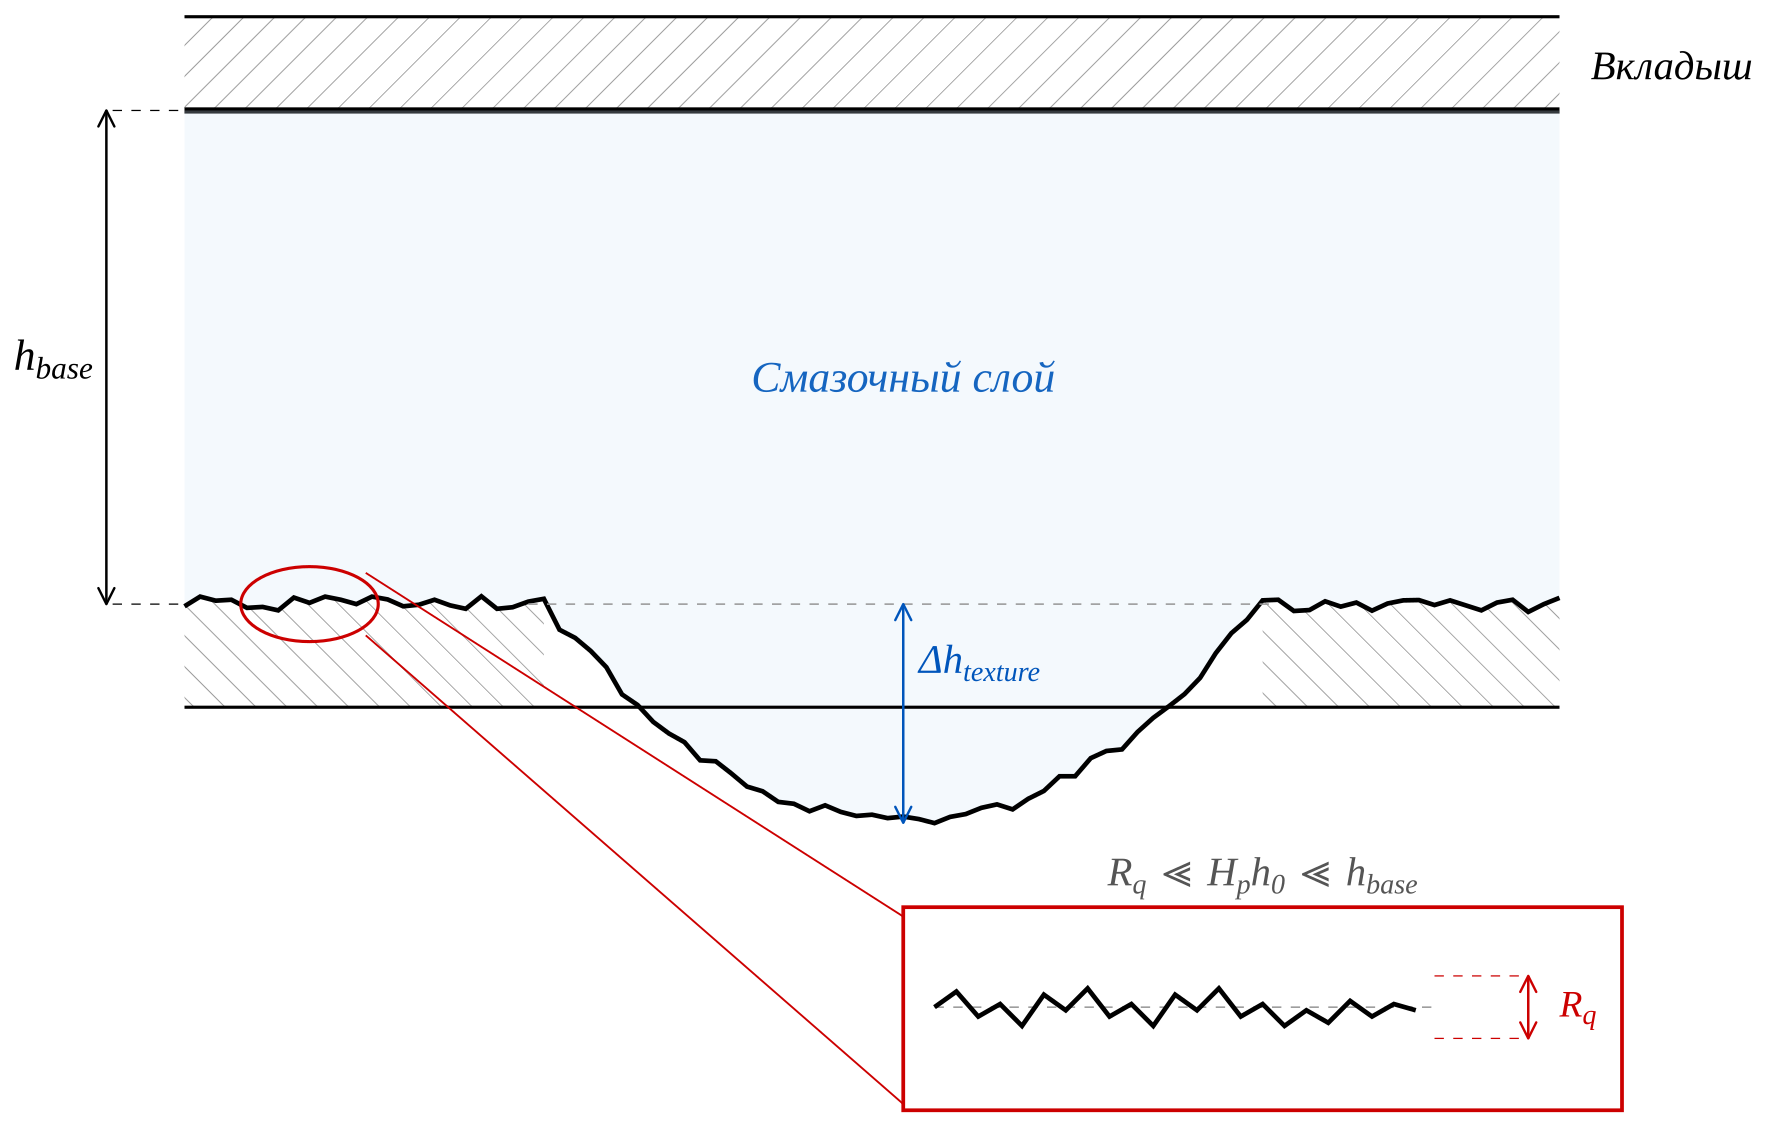
\includegraphics[width=\textwidth,height=0.9\textheight,keepaspectratio]{figures/ch04/fig_4_4.png}
\caption{Иерархия масштабов топографии поверхности:
  базовый зазор, детерминированная микротекстура и шероховатость}
\label{fig:roughness_scales}
\end{figure}

\FloatBarrier

\textit{Подходы к учёту шероховатости в уравнении Рейнольдса.}
В литературе сложились три основных подхода, различающихся
по сложности реализации и области применимости.

Первый подход~-- детерминированный: шероховатость задаётся явным
полем $\Delta h_{\mathrm{rough}}(s_1, s_2)$, полученным по данным
измерений (атомно-силовая микроскопия, контактная профилометрия),
и добавляется в суперпозицию зазора наряду с текстурой:
\[
  h = h_{\mathrm{base}} + \Delta h_{\mathrm{texture}}
    + \Delta h_{\mathrm{rough}}.
\]
Такой подход требует измеренного профиля поверхности
и разрешения расчётной сетки, достаточного для представления
случайного рельефа: шаг сетки должен быть существенно меньше
длины корреляции~$\lambda_c$ (единицы микрометров). Это приводит
к значительному увеличению числа узлов по сравнению с задачей для
гладких поверхностей (глава~3) и обоснованно только в рамках
исследовательских расчётов.

Второй подход~-- стохастический, основанный на осреднении
уравнения Рейнольдса по ансамблю реализаций случайной
шероховатости. Пионерская модель Кристенсена (Christensen, 1969)
и её развитие в работах Патира и Ченга (Patir, Cheng, 1978--1979)
вводят поправочные коэффициенты (\textit{flow factors}), которые
учитывают влияние статистической шероховатости на средние потоки
смазки. Осреднённое уравнение Рейнольдса записывается для
среднего давления~$\bar{p}$ с модифицированными коэффициентами:
\begin{equation}
  \frac{\partial}{\partial s_1}\!\left(\phi_p\,\bar{h}^3\,
  \frac{\partial \bar{p}}{\partial s_1}\right)
  + \Lambda^2\frac{\partial}{\partial s_2}\!\left(\phi_p\,\bar{h}^3\,
  \frac{\partial \bar{p}}{\partial s_2}\right)
  = \phi_s\,\frac{\partial \bar{h}}{\partial s_1}
  + \phi_c\,\sigma_r\,\frac{\partial \phi_s}{\partial s_1}\,,
  \label{eq:reynolds_rough_avg}
\end{equation}
\begin{conditions}
$\bar{h}$ -- номинальная (без случайной составляющей) толщина зазора: $\bar{h} = h_{\mathrm{base}} + \Delta h_{\mathrm{texture}}$ (суперпозиция~\eqref{eq:h_superposition} без~$\Delta h_{\mathrm{rough}}$);\\
$\bar{p}$ -- осреднённое давление;\\
$\phi_p$ -- фактор давления (pressure flow factor),
корректирующий пуазейлевский поток;\\
$\phi_s$ -- фактор сдвига (shear flow factor),
корректирующий куэттовский поток;\\
$\phi_c$ -- контактный фактор;\\
$\sigma_r$ -- суммарная среднеквадратичная шероховатость
контактирующих поверхностей, м ($\sigma_r \equiv R_q$ из~\eqref{eq:lambda_roughness});\\
$\Lambda$ -- отношение масштабов длины
(подраздел~2.1.6).
\end{conditions}
Факторы~$\phi_p$, $\phi_s$ зависят от отношения~$\bar{h}/\sigma_r$
и от ориентации шероховатости (продольная, поперечная,
изотропная). Они вычисляются однократно по статистическим
параметрам поверхности и не требуют разрешения случайного поля
на расчётной сетке, что делает стохастический подход
вычислительно эффективным. Структура
уравнения~\eqref{eq:reynolds_rough_avg} сохраняет форму исходного
уравнения Рейнольдса~\eqref{eq:reynolds_full}, поэтому солверы
и алгоритмы, описанные в главе~3, могут быть адаптированы
с минимальными изменениями. Член с~$\phi_c$ представляет дополнительную поправку, связанную с контактными эффектами при малых значениях~$\lambda_r$; в чисто гидродинамическом режиме ($\lambda_r > 5$) он мал и может быть опущен.

Третий подход~-- пренебрежение шероховатостью: при $\lambda_r \gg 1$
полагается $\Delta h_{\mathrm{rough}} = 0$, и уравнение Рейнольдса
решается для номинального зазора~\eqref{eq:h_superposition}. Это
допущение принято в расчётах глав~5--7 настоящей монографии.

\textit{Взаимодействие шероховатости с детерминированными
микроструктурами.}
При совместном присутствии детерминированных микроструктур
и случайной шероховатости характерные масштабы могут различаться
на порядки. Глубина ячейки микрорельефа~$h_p = H_p \cdot h_0$
составляет, как правило, единицы микрометров (в зависимости от технологии и назначения подшипника) при характерном размере
ячейки в десятки микрометров; шероховатость полированных
поверхностей характеризуется значениями $R_q \sim 0{,}01\text{--}0{,}1$~мкм
при длине корреляции $\lambda_c \sim 1\text{--}10$~мкм.

Когда $R_q \ll H_p \cdot h_0$~-- типичный случай при хорошо
обработанных поверхностях~-- детерминированные микроструктуры
доминируют в формировании поля давления и потоков, а вклад
шероховатости сводится к слабому стохастическому возмущению,
не влияющему на интегральные характеристики подшипника.

Когда $R_q$ оказывается соизмерима с~$H_p \cdot h_0$, что
возможно при грубой обработке или мелком микрорельефе,
шероховатость модифицирует распределение давления внутри ячеек
текстуры, изменяет локальные кавитационные зоны
(раздел~4.1) и может как усилить, так и ослабить эффективность
текстурирования. В этом режиме результаты, полученные в рамках
модели гладких поверхностей, требуют поправок, и корректное
описание предполагает использование одного из рассмотренных выше
подходов~-- детерминированного или стохастического.

Практический вывод для проектирования состоит в том, что
глубина детерминированных микроструктур~$h_p$ должна существенно
превышать среднеквадратичную шероховатость ($H_p \cdot h_0 \gg R_q$),
чтобы регулярный рельеф не терял функциональности на фоне случайных
микронеровностей. Это условие одновременно обеспечивает
$\lambda_r \gg 1$, при котором пренебрежение шероховатостью
в уравнении Рейнольдса обосновано.

В расчётах глав~5--7 поверхности приняты гладкими:
$\Delta h_{\mathrm{rough}} = 0$. Допущение оправдано при
$\lambda_r \gg 1$ и $H_p \cdot h_0 \gg R_q$, что типично
для прецизионных подшипников с полированными поверхностями.
Стохастический подход с коэффициентами потоков~$\phi_p$,
$\phi_s$~\eqref{eq:reynolds_rough_avg} представляет наиболее
практичный путь расширения модели на случай существенной
шероховатости: он сохраняет структуру дискретизации и не требует
разрешения случайного поля на расчётной сетке.
Детерминированный подход применим при наличии измеренных профилей
поверхности и вычислительных ресурсов для высокого разрешения
сетки, характерного масштаба $\lambda_c$.
При необходимости кавитация учитывается постановкой JFO для осреднённого давления~$\bar{p}$, т.\,е.\ условия комплементарности~\eqref{eq:jfo_complementarity} применяются к уравнению~\eqref{eq:reynolds_rough_avg}~\cite{gu2017,nie2022}.

\textit{Физический смысл коэффициентов потока Патира--Ченга.}
В модели Патира--Ченга~\cite{patir1978} исходное уравнение
Рейнольдса заменяется осреднённым уравнением с коэффициентами
потока $\phi_x$, $\phi_y$ (по давлению) и $\phi_s$ (по сдвигу):
%
\begin{equation}
  \frac{\partial}{\partial x}\!\left[\phi_x\,\bar{h}^3\,
  \frac{\partial \bar{p}}{\partial x}\right]
  + \frac{\partial}{\partial y}\!\left[\phi_y\,\bar{h}^3\,
  \frac{\partial \bar{p}}{\partial y}\right]
  = 6\mu U\,\frac{\partial}{\partial x}\!\left(\bar{h}
  + \phi_s\,\sigma_{\mathrm{eq}}\right).
  \label{eq:patir_cheng}
\end{equation}
%
Коэффициент $\phi_s$ описывает дополнительный перенос смазки
за счёт шероховатости (неоднородности переносного потока),
а $\phi_x$, $\phi_y$ отражают анизотропное сопротивление
шероховатости напорному потоку. Все три коэффициента зависят
от параметра $\lambda_r = \bar{h}/\sigma_{\mathrm{eq}}$
и ориентации шероховатости (изотропная, продольная,
поперечная). При $\lambda_r \gg 1$ все коэффициенты стремятся
к единице и уравнение~\eqref{eq:patir_cheng} вырождается
в классическое уравнение Рейнольдса.
При $\lambda_r < 3$ поправки становятся существенными:
$\phi_x$ и $\phi_y$ снижаются ниже единицы (шероховатость
затрудняет напорное течение), тогда как $\phi_s$ может
превышать единицу или быть меньше в зависимости от ориентации.

\textit{Обоснование допущения о гладких поверхностях.}
Допущение о гладких поверхностях ($\phi_x = \phi_y = 1$,
$\phi_s = 0$) принято в прикладных расчётах настоящей работы.
Его обоснование: параметр
$\lambda_r = h_{\min}/\sigma_{\mathrm{eq}}$ в характерных
режимах составляет $\lambda_r \geq 2$ (смешанный режим),
при котором поправки Патира--Ченга имеют ограниченное влияние
на интегральные характеристики и слабо меняют сравнительный
вывод о преимуществе текстурированного варианта над гладким.
Кроме того, детерминированная текстура (глубина
$H_p = 0{,}2$--$0{,}4$ в единицах зазора) по амплитуде
существенно превосходит стохастическую шероховатость
(характерная высота
$\sigma_{\mathrm{eq}} \ll h_{\min}$), поэтому вклад
случайного микрорельефа в интегральные характеристики
подшипника значительно меньше вклада детерминированных лунок.
Включение модели Патира--Ченга потребовало бы ввода
дополнительных параметров (тип и ориентация шероховатости,
коэффициенты потока), которые выходят за рамки исследуемых
переменных, не изменяя качественных выводов работы.
